The Parkinson's Progression Markers Initiative (PPMI) dataset, which is openly available, includes a diverse range of data such as T1-Weighted MRI scans, demographic information, 
and clinical assessment records for participants enrolled in the study. In our research, we curated specific cohorts from the PPMI dataset, employing the Hoehn and Yahr Scale (H\&Y) 
to assess the progression of Parkinson's disease among subjects. Further demographic features were extracted from the study files and radiomic features were derived from the T1-Weighted 
MRI scans. These served as inputs for the training of several machine learning models. During the model training phase, a feature selection process was applied to extract the most 
pertinent features. The effectiveness of the models was evaluated using the Area Under the Receiver Operating Characteristic (ROC) Curve (AUC) as a scoring metric. 
Fig~\ref{modelOverview} provides a schematic representation of our analytical workflow, encapsulating the sequence of processes from data extraction to model evaluation.

\begin{figure}[!ht]
    \centering
    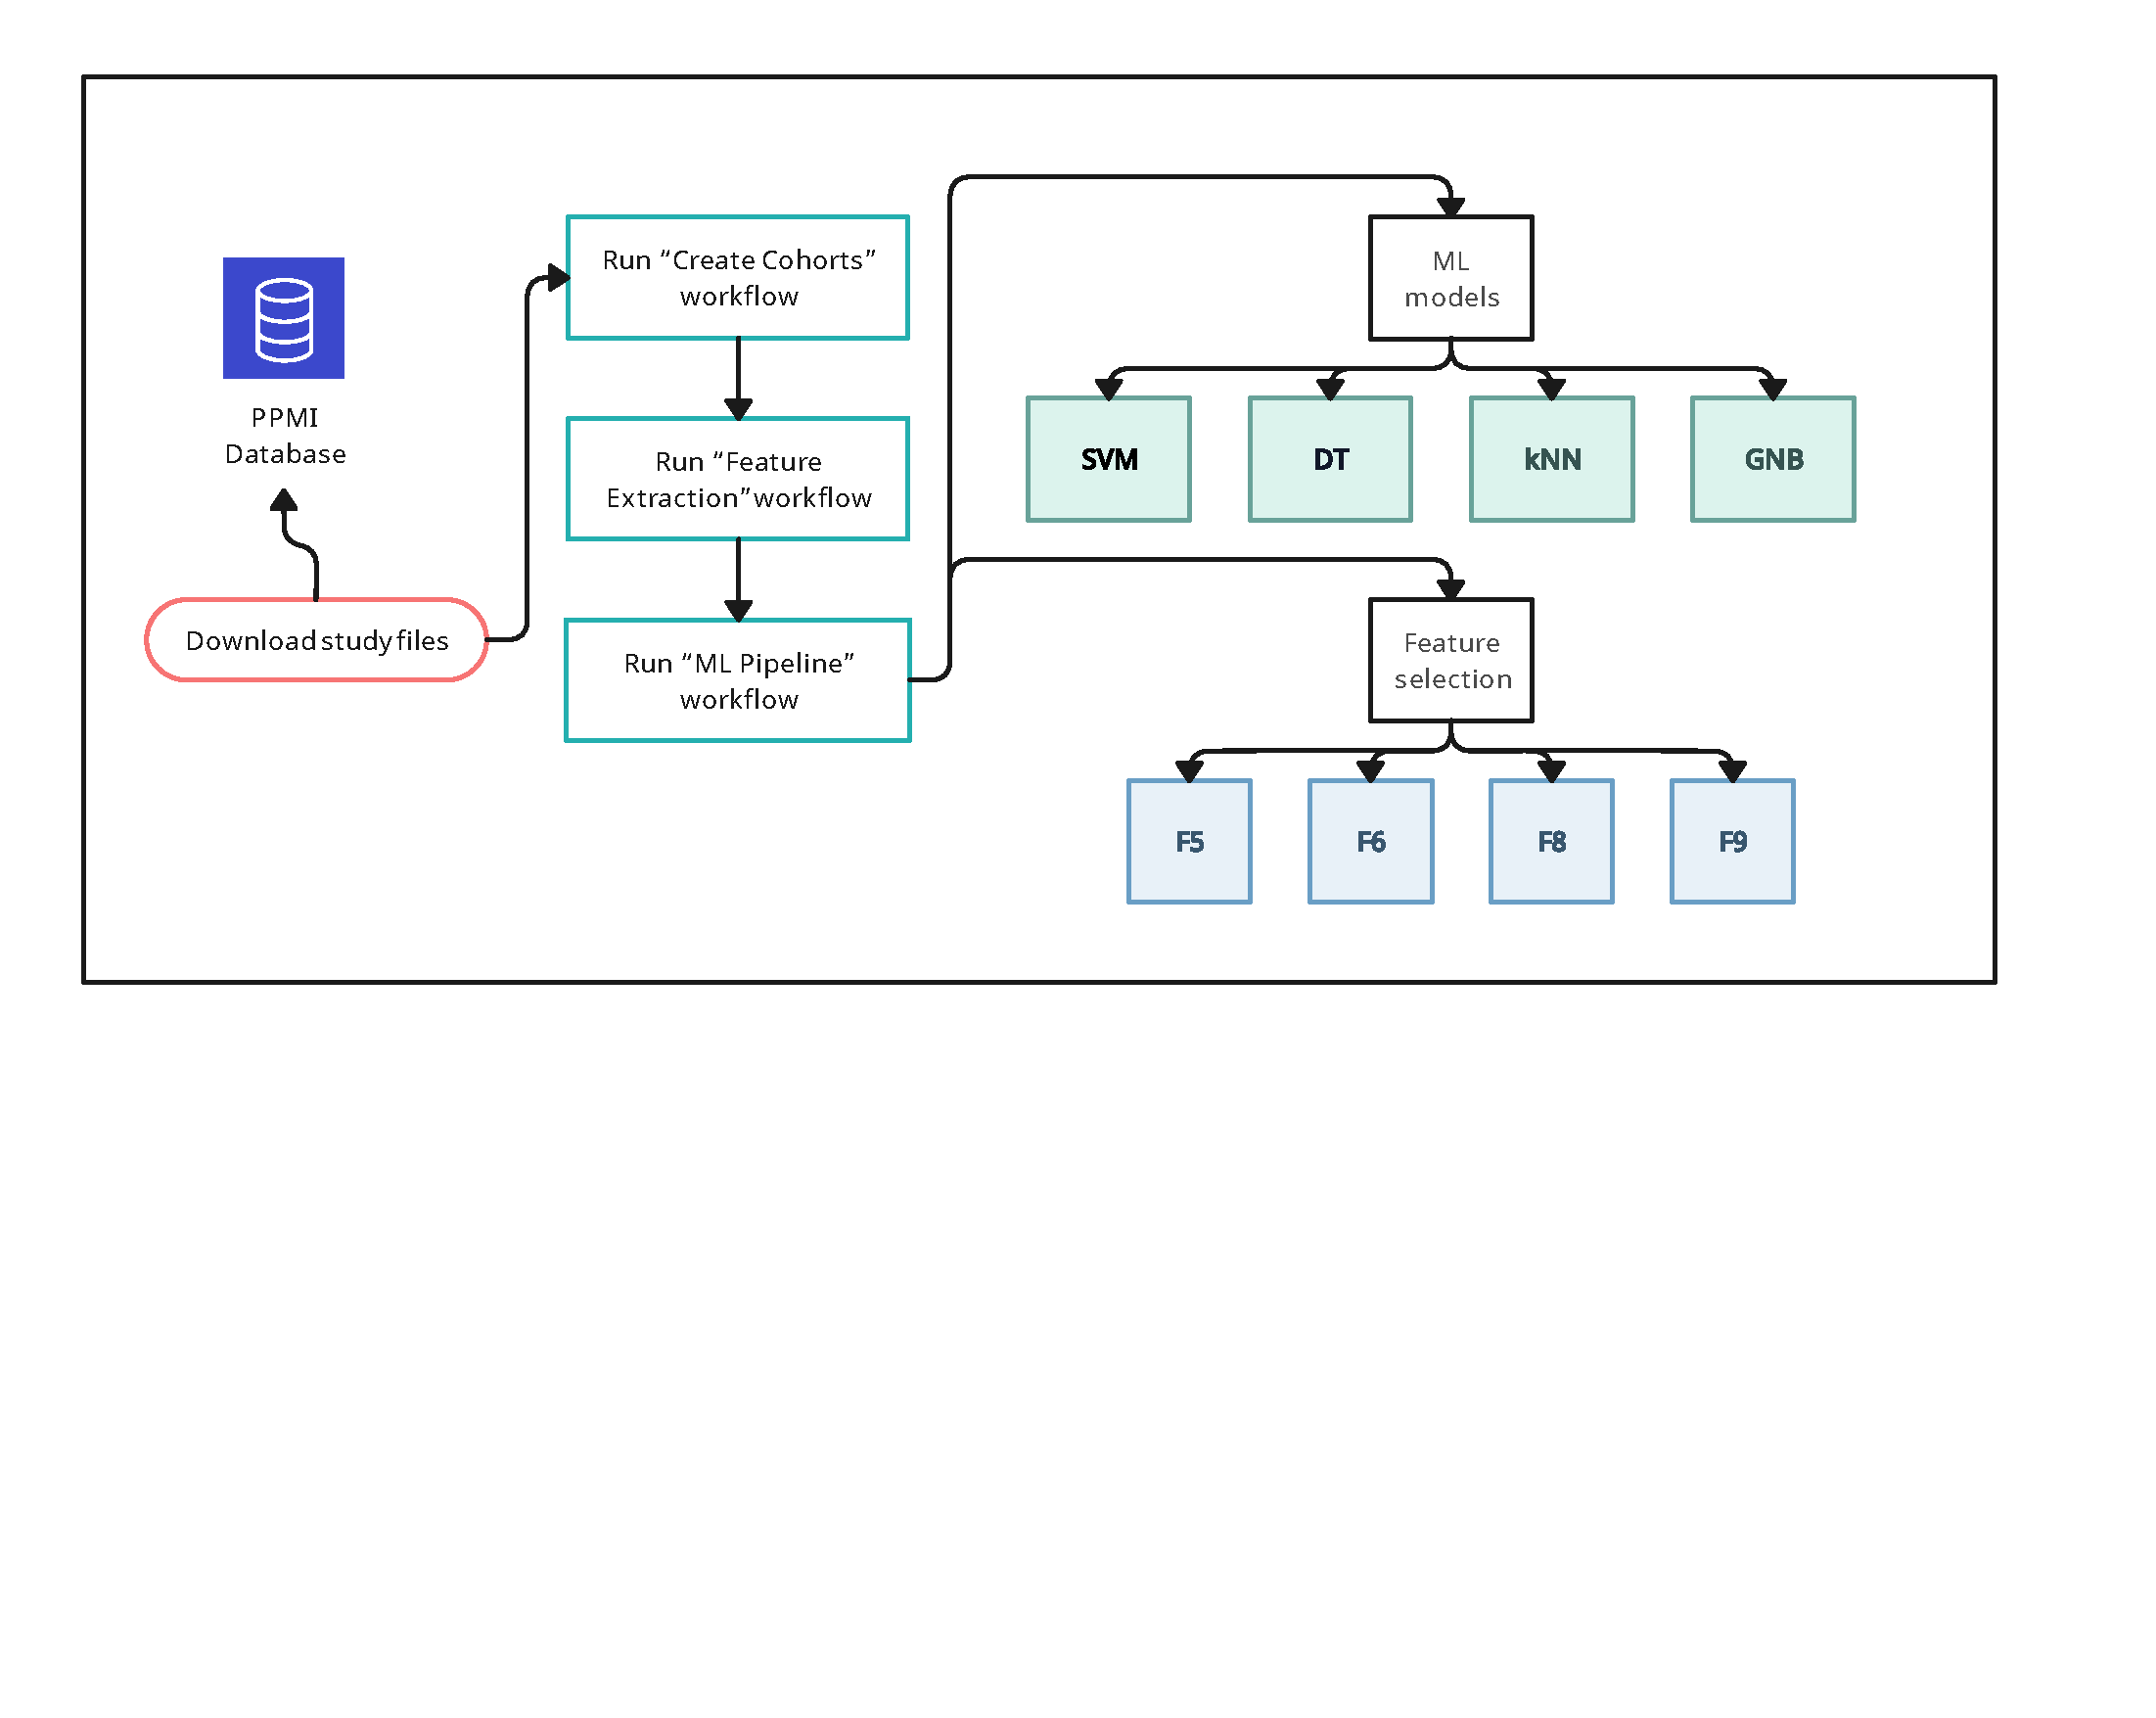
\includegraphics[trim=0 320 0 0, clip, width=\linewidth]{images/Methods_workflow.pdf}
    \caption{Workflow: The process begins with downloading the study files from the PPMI database, using the patient data to create cohorts, extracting the radiomic as well as the 
    demographic features, then training the machine learing models and performing feature selection. See Fig~\ref{cohortCreationFlowchart} for the "Create Cohorts" workflow. See 
    Fig~\ref{featureExtraction} for the "Feature Extraction" workflow. See Fig~\ref{mlPipeline} for the "ML Pipeline" workflow. }
    \label{modelOverview}
\end{figure}
